\port
\section*{Abstract ão}
\par Osteogenesis imperfecta (OI) is a family of genetic disorders associated with
                    bone loss and fragility. Mutations associated with OI have been found in genes
                    encoding the type I collagen chains. People with OI type I often produce
                    insufficient α1-chain type I collagen because of frameshift, nonsense, or splice
                    site mutations in \textit{COL1A1} or \textit{COL1A2}. This
                    report is of a Chinese daughter and mother who had both experienced two bone
                    fractures. Because skeletal fragility is predominantly inherited, we focused on
                    identifying mutations in \textit{COL1A1} and \textit{COL1A2}
                    genes. A novel mutation in \textit{COL1A1}, c.700delG, was detected by
                    genomic DNA sequencing in the mother and daughter, but not in their relatives.
                    The identification of this mutation led to the conclusion that they were
                    affected by mild OI type I. Open reading frame analysis indicated that this
                    frameshift mutation would truncate α1-chain type I collagen at residue p263
                    (p.E234KfsX264), while the wild-type protein would contain 1,464 residues. The
                    clinical data were consistent with the patients’ diagnosis of mild OI type I
                    caused by haploinsufficiency of α1-chain type I collagen. Combined with previous
                    reports, identification of the novel mutation
                        \textit{COL1A1-}c.\textit{700delG} in these patients
                    suggests that additional genetic and environmental factors may influence the
                    severity of OI.

\par \noindent \\
\textit{Keywords}: Osteogenesis imperfecta, Chinese OI type 1 family, type I collagen, sequence analysis, frameshift mutation
\par \noindent \\
Received: 01/12/2013; Accepted: 09/08/2014.\par \noindent \\
\section*{Introduction}\par Osteogenesis imperfecta (OI), also known as brittle bone disease (Marini \textit{et al.}, 2007), is a group of rare
                heritable connective tissue disorders characterized by skeletal fractures with mild
                trauma, secondary deformities, and extraskeletal manifestations (Ben Amor \textit{et al.}, 2011; Marini \textit{et al.}, 2007). Such
                manifestations may include blue sclerae, progressive hearing loss, dentinogenesis
                imperfecta, and hyperlaxity of ligaments and skin (Ben Amor \textit{et al.}, 2011; Marini \textit{et al.}, 2007). The prevalence of OI ranges from
                1 in 10,000 to 1 in 25,000 (Byers and Cole,
                    2002).\par OI was originally classified into four clinical types, I–IV, based on its clinical
                features and radiographs (Sillence \textit{et
                        al.}, 1979; Table S1). Type V has been associated with hyperplastic
                callus formation (Glorieux \textit{et al.},
                    2000), type VI with a mineralization defect (Glorieux \textit{et al.}, 2002) and type VII with
                a range of severity that may be lethal (Ward
                        \textit{et al.}, 2002). OI types VIII and IX are usually
                lethal (Barnes \textit{et al.}, 2012;
                    Moul \textit{et al.}, 2013). OI
                severity ranges from intrauterine fractures and perinatal lethality to extremely
                mild forms without fractures (Ben Amor \textit{et
                        al.}, 2011). The severity of bone fragility of OI patients is
                highest in types VIII and IX, and declines progressively from type II to type VII.
                Type I exhibits the least severe fragility (Rauch
                    and Glorieux, 2005). Most OI types (I–VI) show autosomal dominant
                inheritance, but two of the rarer types (VII and VIII) exhibit autosomal recessive
                disorders (Ward \textit{et al.},
                2002; Ben Amor \textit{et al.},
                    2011; Table
                    S1).\par Type I collagen fibers contain three polypeptide chains. The vast majority of fibrils
                are composed of two α1 and one α2 chains, but a small number are composed of three
                α1 chains in a triple helix structure. The translated collagen α chains include
                propeptides at each end, one at the amino terminus end and one at the carboxyl
                terminus end. These propeptides help to connect and arrange the three chains which
                subsequently interwine in a zipper-like fashion into the triple helix
                configuration.\par Most patients with types I–IV OI (90\%) have a mutation in one of the two collagen
                type I genes, \textit{COL1A1} or \textit{COL1A2} (Ben Amor \textit{et al.}, 2011; van Dijk \textit{et al.}, 2012; Table S1).
                    \textit{COL1A1} extends 18 kb from 17q21.33 to 17q22 and has 52 exons.
                    \textit{COL1A2} extends 37 kb from 7q21.3 to 7q22.3 and has 52 exons.
                More than 200 mutations in collagen 1 genes have been associated with OI (Ben Amor \textit{et al.}, 2011). These
                mutations occur in most exons and introns of \textit{COL1A1} and
                    \textit{COL1A2} (http://www.le.ac.uk/ge/collagen/; Dalgleish, 1997, 1998).\par Many OI type I patients have \textit{COL1A1} and \textit{COL1A2}
                frameshift mutations, splice site mutations, and insertion mutations resulting in
                haploinsufficiency, or the expression of approximately half the amount of collagen
                type I mRNA and protein, leading to weaker bones (Redford-Badwal \textit{et al.}, 1996; Slayton \textit{et al.}, 2000; Peng \textit{et al.}, 2012). Other deletions,
                insertions, and point mutations in \textit{COL1A1} or
                    \textit{COL1A2} induce conformational changes in the collagen α1 and α2
                chains and lead to knot microfibril structure disorders, altered deposition of
                hydroxyapatite, brittleness, reduced resistance to external force, altered stability
                of the collagen triple helix, and fragility (Pallos
                        \textit{et al.}, 2001; Witecka \textit{et al.}, 2008; Ben Amor \textit{et al.}, 2011).\par Clinical diagnosis of osteogenesis imperfecta is straightforward in individuals with
                a positive family history and several typical OI features (van Dijk \textit{et al.}, 2012). However, despite
                the presence of several physical manifestations, some patients are difficult to
                diagnose in the absence of an affected family member and without apparent
                association between bone frailty and obvious extraskeletal abnormalities. In these
                cases, analyses of type I collagen genes for mutations can provide helpful
                information since 90\% of OI-associated mutations arise in collagen I (van Dijk \textit{et al.}, 2012).\par Here, we present the results of \textit{COL1A1} and \textit{COL1A2}
                sequencing analysis from DNA samples collected from two related Chinese patients
                with several typical features of OI. A novel mutation not previously associated with
                    \textit{COL1A1} was detected. These results will help to provide a
                better diagnosis of mild OI type I when physical symptoms are mild.\section*{Materials and Methods}\subsection*{Patients}\par Two related Han Chinese patients, mother and daughter, presented with blue
                    sclerae, bone pain, and dentinogenesis imperfecta. Each had experienced two bone
                    fractures. We reviewed their clinical features, medical history, physical
                    examination, radiologic images, and biochemical parameters, and diagnosed them
                    with type I osteogenesis imperfecta. Both affected family members, unaffected
                    family members (maternal grandmother, father, and two sisters), and controls
                    agreed to a genetic analysis and provided informed consent for the study
                    approved by the Endocrinology Department of General Hospital of PLA. Their
                    pedigree is shown in Figure 1.
\begin{figure}[p]
\centering
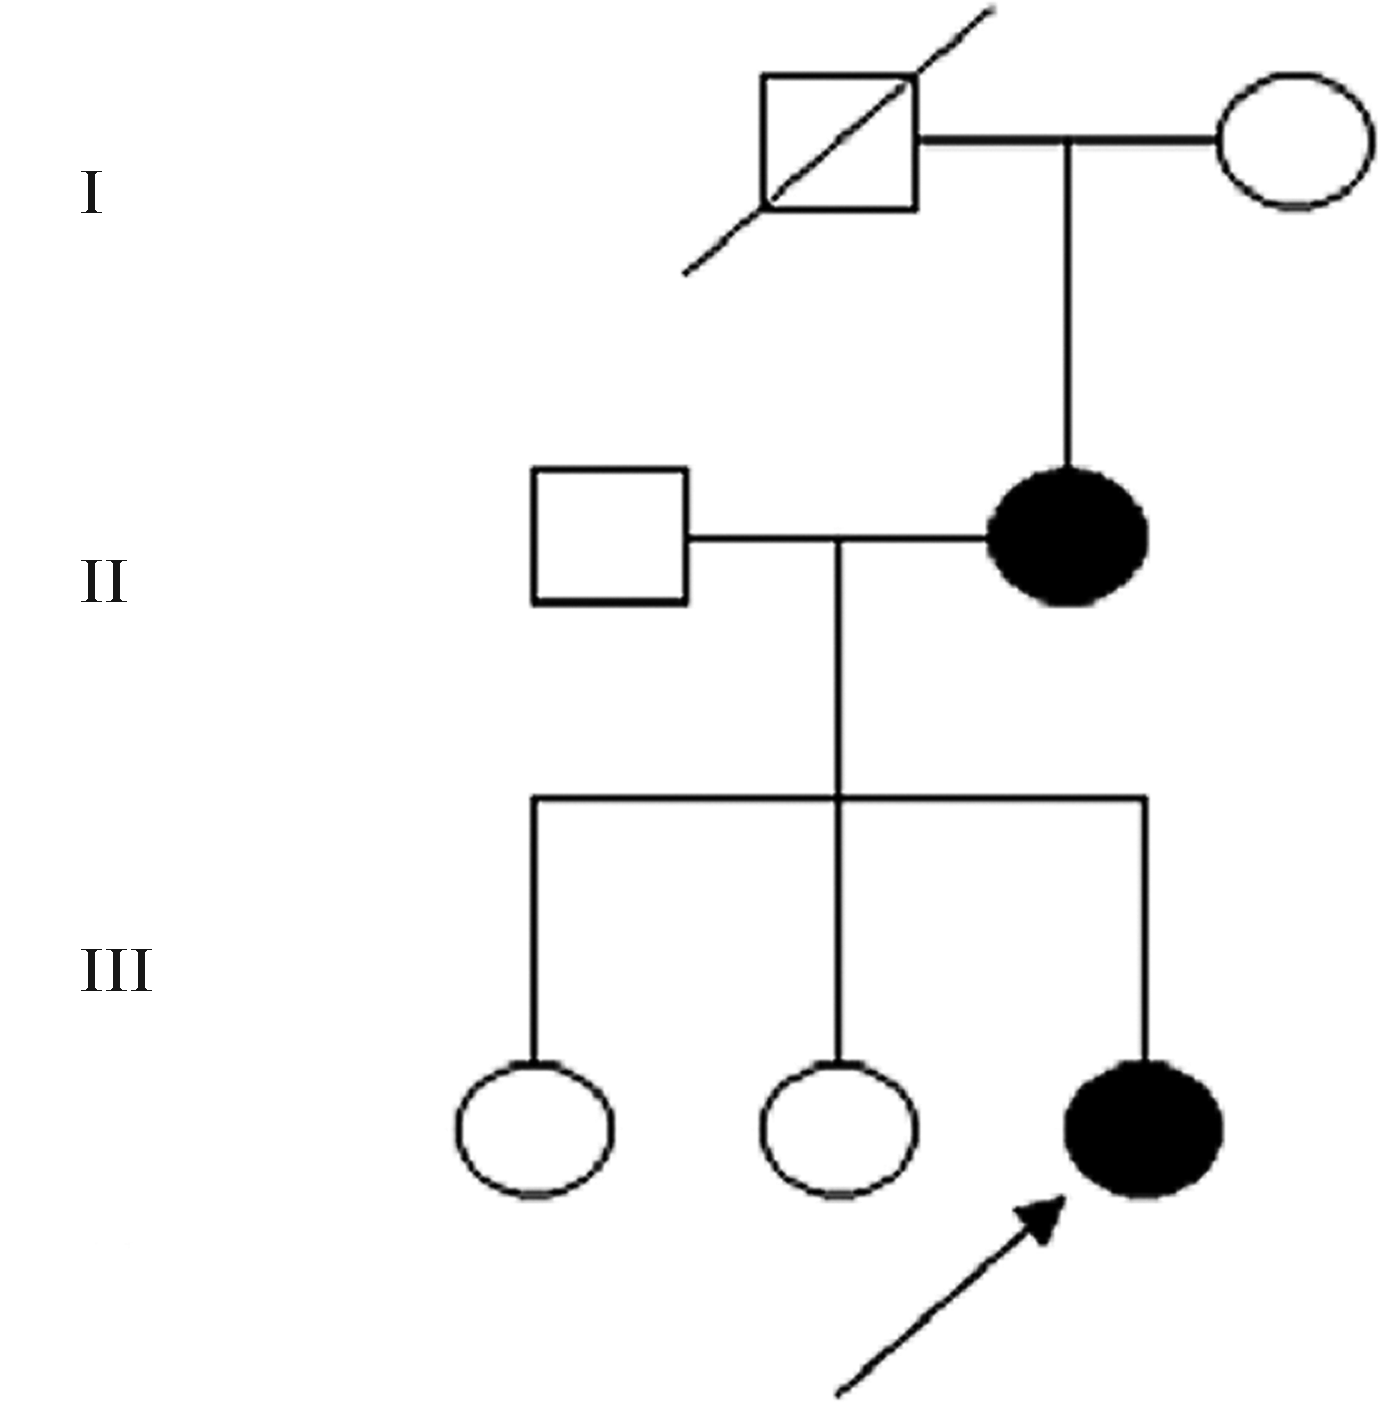
\includegraphics[width=0.5\textwidth]{1415-4757-gmb-38-1-1-gf01.png}
\caption{The osteogenesis imperfecta pedigree of the nuclear family of the
                            proband.}
\label{Figure 1}
\end{figure}

\subsection*{Genetic analysis}\par Blood samples were obtained from the two patients, their family members, and 50
                    ethnically matched, unrelated controls. Genomic DNA was isolated from peripheral
                    leukocytes by using a whole blood DNA extraction kit (Qiagen Co., Valencia, CA)
                    according to the manufacturer’s instructions. PCR was performed to detect
                    sequences in all exons and exon-intron boundaries of \textit{COL1A1} and
                        \textit{COL1A2}. Fifty-seven pairs of primers, 17 for
                        \textit{COL1A1} and 40 for \textit{COL1A2} (sequences
                    available upon request), were designed and verified with Primer 5 software
                    (Softonic, Shanghai, China) using the genomic sequences of
                        \textit{COL1A1} (GenBank accession NG\_007400.1) and
                        \textit{COL1A2} (Genbank accession NG\_007405.1).\par DNA sequence analysis was performed by automated sequencing in an ABI genetic
                    analyzer (Model 377; ABI, USA) by the Ying Jun Gene Company (Shanghai, China).
                    Sequencing results were compared with the GenBank database and confirmed through
                    sequencing of clones. DNA was cloned into a PGEM-T Easy Vector following the
                    manufacturer’s instructions (Promega, Madison, WI). The osteogenesis imperfecta
                    and Ehlers-Danlos syndrome variant databases compiled of previously reported OI
                    mutations in \textit{COL1A1} and \textit{COL1A2}, the 1000
                    Genomes database, and the UniProKB database were also used for comparison. PCR
                    and sequencing of \textit{COL1A1} and \textit{COL1A2} genes in
                    samples of other family members were performed with the same methods.\par Open reading frame analysis of the mutated sequence was performed by the ORF
                    Finder, part of the BLAST software suite. The parental protein sequence and the
                    protein sequence corresponding to the c.700delG mutation were aligned using the
                    align function of BLAST software (NCBI). The 1000 Genomes database was also used
                    to search for the presence of this mutation by using the alignment function of
                    the BLAST software and the following search sequence: 5′-TTTTCTCTCCCTCTCAGGGGA
                    AGCTGGAAAACCTGGT CGTCCTGGTGAGCG-3′.\section*{Results}\subsection*{Patient description}\par The proband was a 13-year-old girl of Han descent from the Shanxi province of
                    China. Her spontaneous full-term delivery was uneventful. The proband began
                    walking at 15 months. She had suffered two bone fractures in the long bone and
                    vertebra. The first fracture occurred in the right tibia/fibula after a slight
                    injury at 16 months old and its healing was achieved with fixation of a plate.
                    The second fracture was caused by a slight hit to the abdomen. The proband did
                    not grow in height during the last two years. Mental development was normal.
                    Physical examination revealed short stature, blue sclerae, discrete signs of
                    dentinogenesis imperfecta, pigeon breast, deformities of slight scoliokyphosis
                    and joint hypermobility. X-rays showed thoracic-lumbar vertebra compression
                    fracture and osteoporosis, acetabulum, and femoral head protrusion acetabulum
                    into the pelvis.\par The mother is a 43-year-old of Han Chinese descent. She had two fractures in
                    childhood: one in the right tibia/fibula that occurred at age 5 and the other in
                    the right radius at age 8. She presented with hearing loss that had onset near
                    the age of 20. Physical examination revealed blue sclerae, discrete signs of
                    dentinogenesis imperfecta, deformity of scoliosis, and joint hypermobility.
                    Blood samples were analyzed from the two patients and blood serum calcium,
                    phosphorus, and parathyroid hormone levels were all within the normal range
                    (data not shown).\subsection*{Mutation analysis}\par Sequence analysis revealed no mutations in the \textit{COL1A2} gene from
                    the proband or her mother. However, sequence analysis of \textit{COL1A1}
                    identified a heterozygous frameshift mutation in exon 10 from both subjects at
                    nucleotide 700 of the mRNA, named as c.700delG, with nucleotide 1 defined as A
                    of the initiating ATG (Figure 2). This
                    mutation was not identified in other family members (two sisters, father, and
                    maternal grandmother of the proband) or ethnically matched controls.
                    Importantly, a comparison with the compiled list of \textit{COL1A1}
                    mutations associated with OI in the osteogenesis imperfecta and Ehlers-Danlos
                    syndrome variant databases (Dalgleish,
                        1997, 1998 and http://www.uniprot.org/uniprot/P02452a) revealed that the
                    mutation is novel and had not been previously reported.
\begin{figure}[p]
\centering
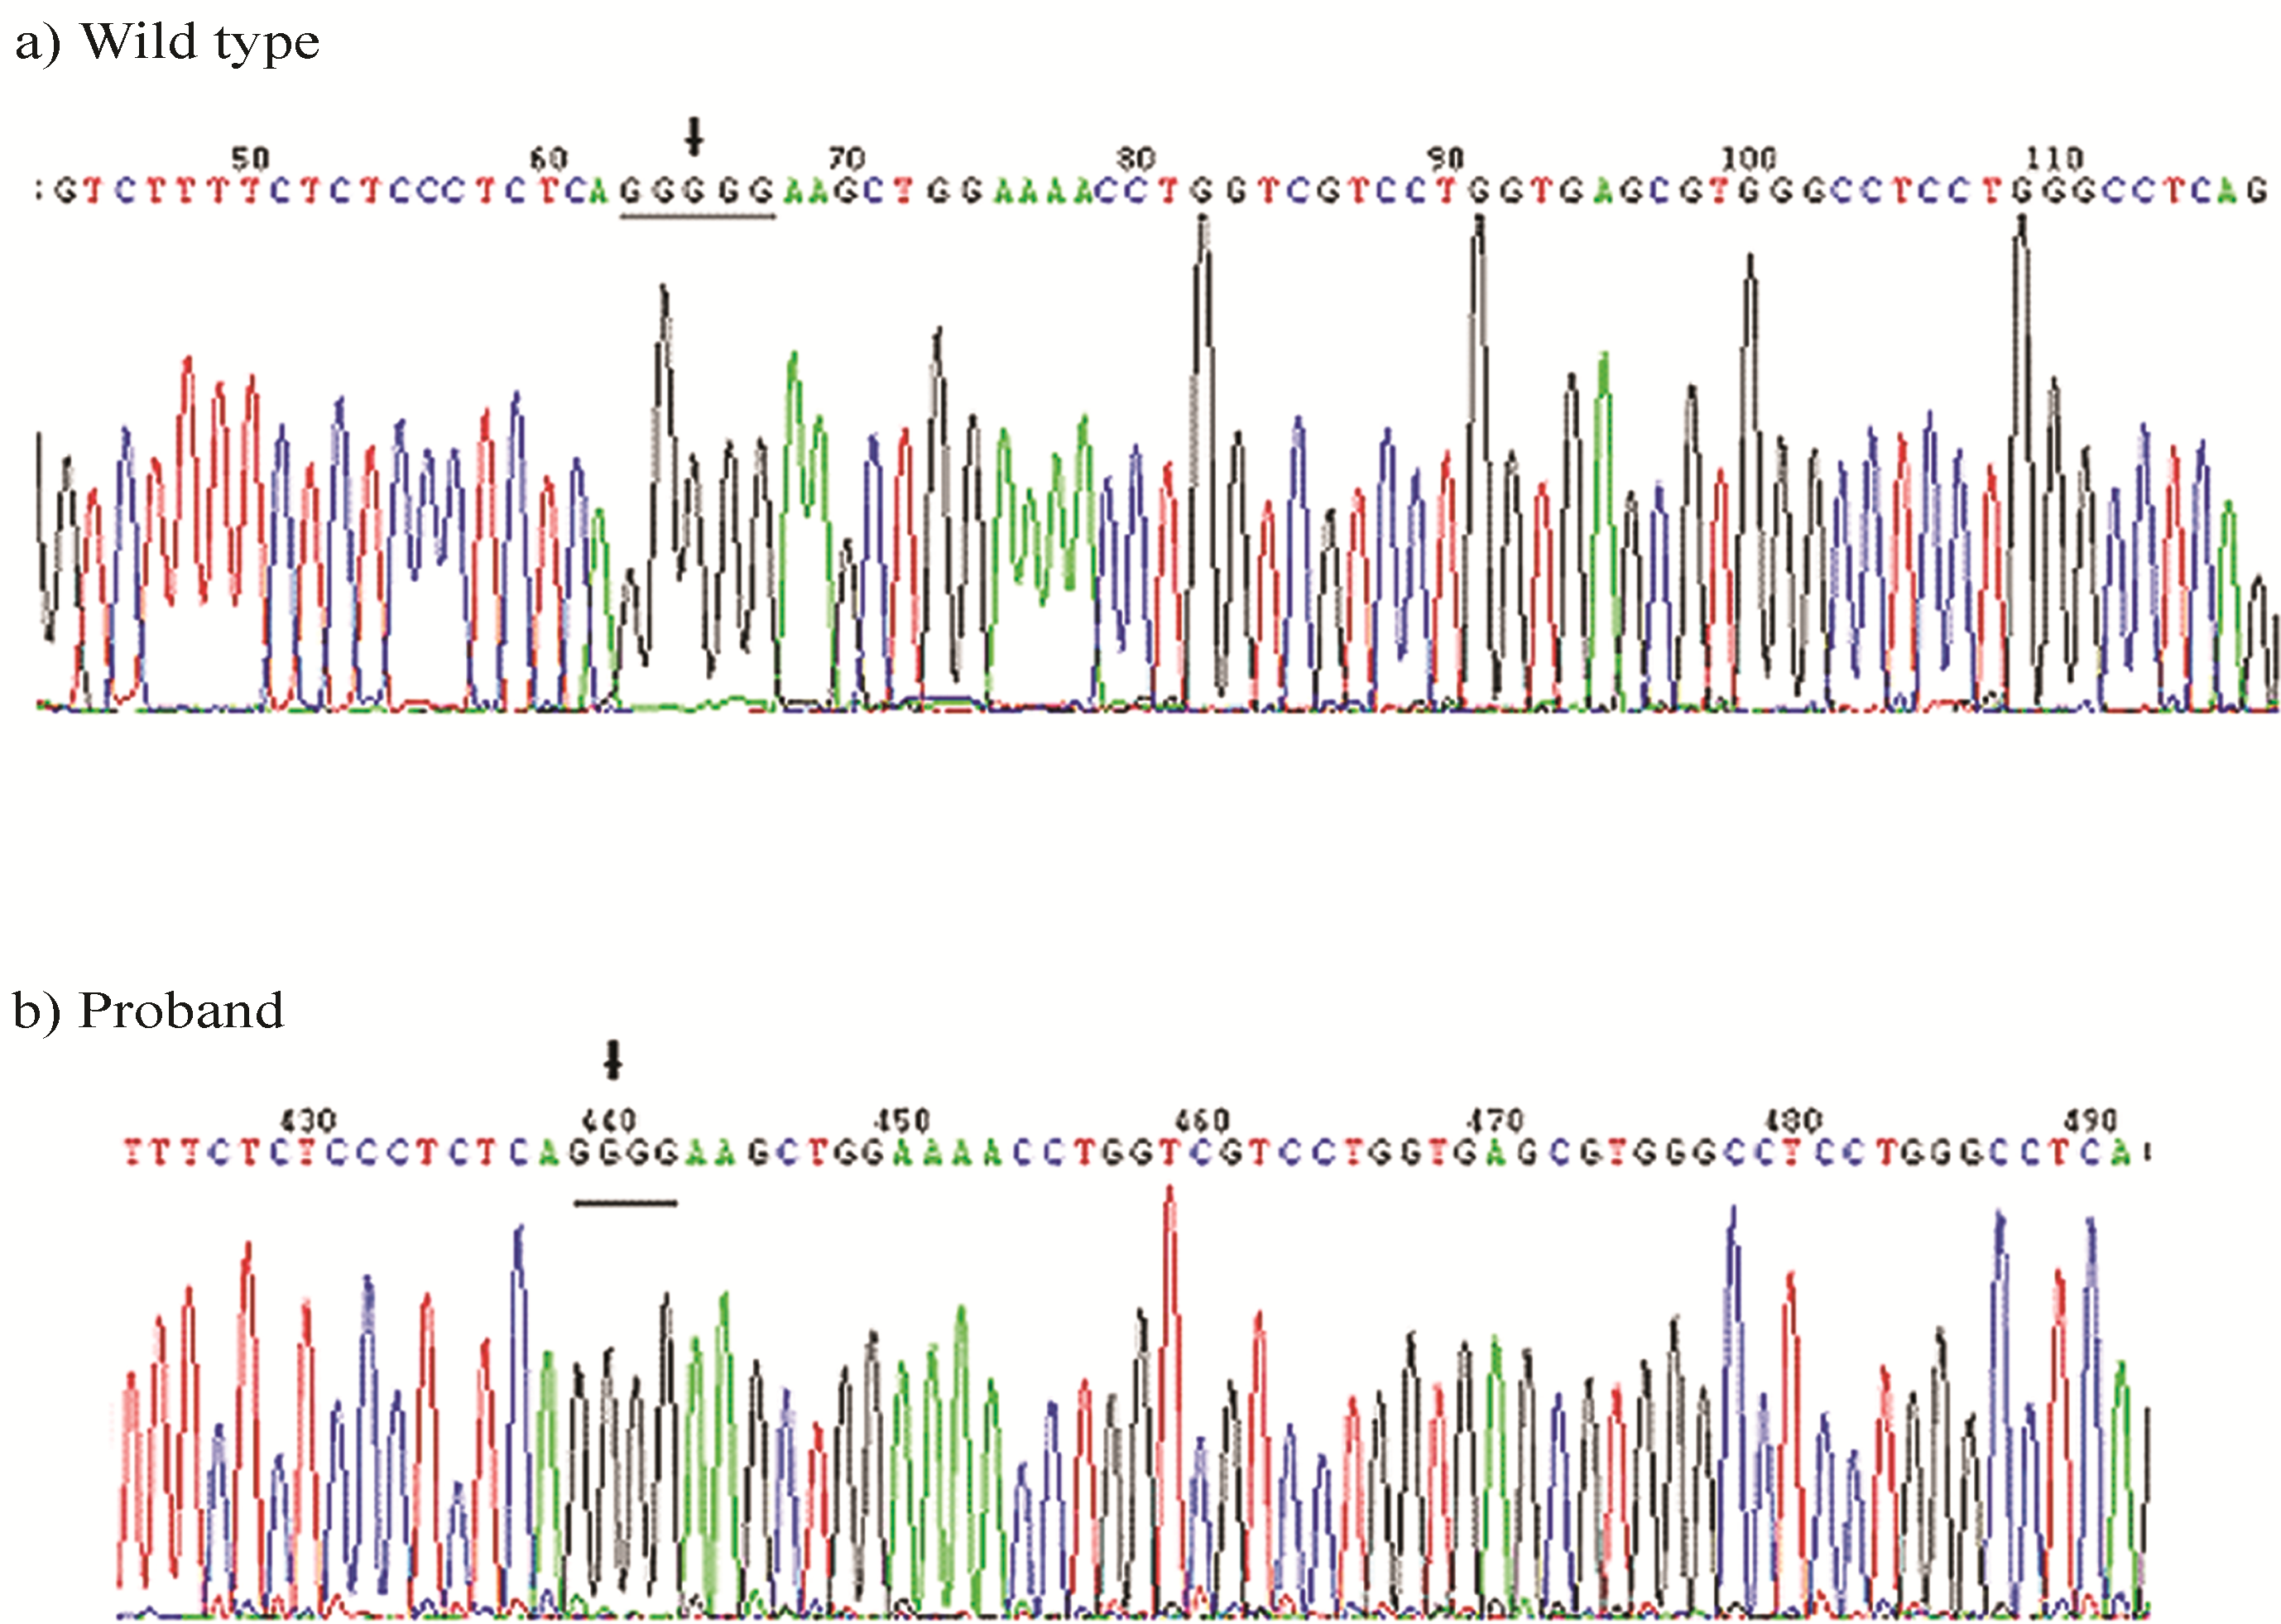
\includegraphics[width=0.5\textwidth]{1415-4757-gmb-38-1-1-gf02.png}
\caption{Sequence analysis of \textit{COL1A1} from a wild-type control
                            and the same DNA region from the proband containing the mutation. DNA
                            sequencing was initiated in the ninth intron and extended into the tenth
                            exon. (A) Genomic DNA sequence of the control wild-type allele. (B) DNA
                            sequence of a \textit{COL1A1} clone from the proband. The DNA
                            sequence of the same region from the mother was identical to the proband
                            (data not shown).}
\label{Figure 2}
\end{figure}

\par This novel, heterozygous c.700delG frameshift mutation in \textit{COL1A1}
                    was inherited in an autosomal dominant manner and was correlated with OI
                    symptoms (Figure 2). An open reading frame
                    (ORF) analysis indicated that translation of the
                        \textit{COL1A1-}c.\textit{700delG} mRNA would initiate at
                    the standard methionine and would be 100\% homologous until amino acid 233.
                    However, the mutation would produce distinct amino acids from p234 to p263 when
                    compared to wild-type collagen α1 and would terminate at the UGA stop codon at
                    nucleotide 792 in exon 10 (Figure 3). This
                        \textit{COL1A1} mutation would be named p.E234KfsX264. According to
                    the ORF analysis, the putative 263 amino acid collagen α1 700delG mutation would
                    contain the signal peptide (p1–22), propeptide (p23–161) and the first 102
                    residues of the main collagen α1 chain (p162–1218 and the triple helical region
                    from p179–1192), but no C-terminal propeptide (p1219–1464). Thus, the mutation
                    produces a truncated form of COL1A1. The second allele was normal in the proband
                    and mother. The mutation was not described in genomes submitted to the 1000
                    Genomes database.
\begin{figure}[p]
\centering
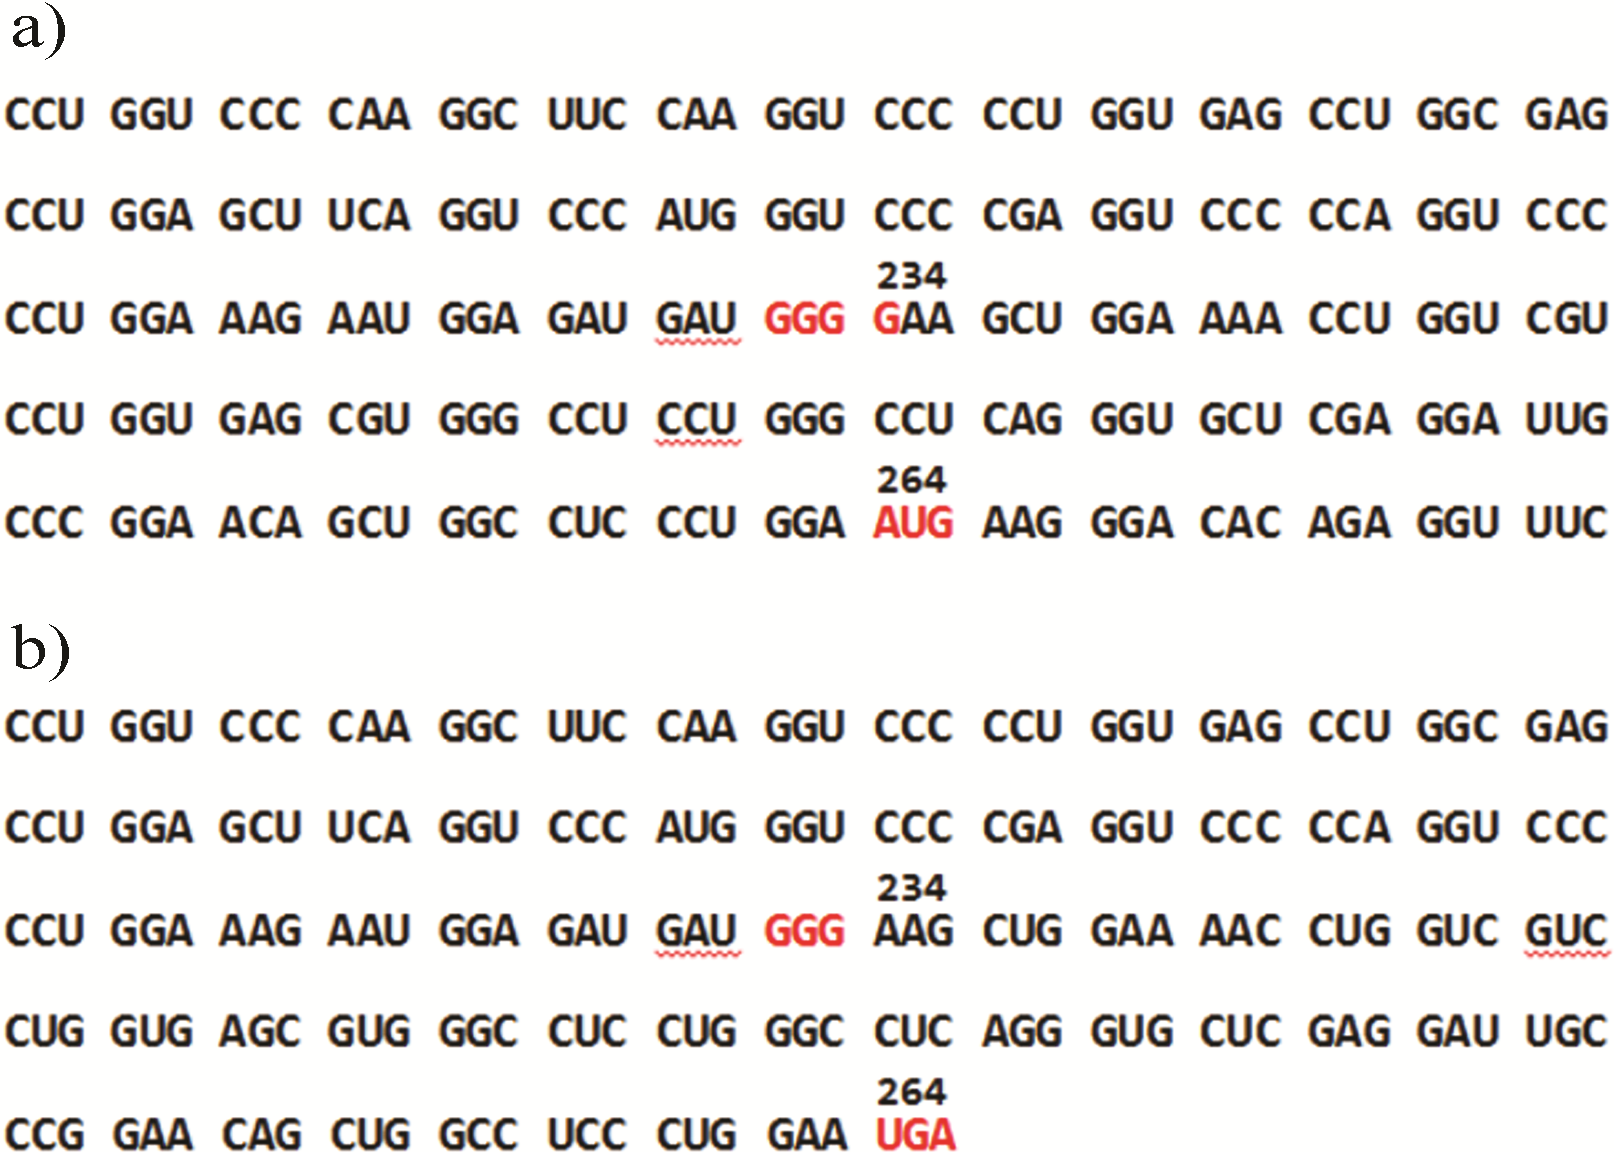
\includegraphics[width=0.5\textwidth]{1415-4757-gmb-38-1-1-gf03.png}
\caption{Comparison of mRNA sequences from the wild-type control and proband.
                            The mRNA sequence is shown from nucleotide 586 (codon 196) in exon 9 to
                            nucleotide 810 (codon 270) in exon 10 with nucleotide 1 defined as the A
                            of the AUG/ATG translational start codon. The splicing of introns
                            between exon 9 and 10 removed the first G of a five-G sequence in the
                            parental cDNA, providing four Gs from nucleotide c.697–700, whereas the
                            proband mutant \textit{COL1A1} mRNA only contained a 3-G
                            sequence. This c.700delG genotype induced a frameshift mutation in the
                            proband and her mother. (A) Wild-type \textit{COL1A1} mRNA. (B)
                            Proband \textit{COL1A1} mRNA with the 700delG variant.}
\label{Figure 3}
\end{figure}

\section*{Discussion}\par Mutations in \textit{COL1A1} and \textit{COL1A2} account for
                approximately 90\% of OI cases and usually occur in patients with OI types I–IV. OI
                symptoms can also occur in patients with mutations in genes that code proteins that
                interact with type I collagen, including cartilage associated protein (CRTAP; Starman \textit{et al.}, 1989; Barnes \textit{et al.}, 2006; Morello \textit{et al.}, 2006; Valli \textit{et al.}, 2012),
                prolyl-3-hydroxylase 1 (P3H1/LEPRE1), cyclophillin B (PPIB; Morello \textit{et al.}, 2006; Fratzl-Zelman \textit{et al.}, 2010; Marini \textit{et al.}, 2010; Valli \textit{et al.}, 2012; Zhang \textit{et al.}, 2012), FKBP10
                    (Barnes \textit{et al.}, 2012),
                WNT-1 (Pyott \textit{et al.}, 2013),
                and serpin peptidase inhibitor clade F member 1 (SERPINF1, Homan \textit{et al.}, 2011). In our report, the
                clinical presentation of OI in the proband and her mother was mild, and the
                associated finding of a frameshift mutation in both patients allowed diagnosis of
                type I osteogenesis imperfecta.\par Many patients diagnosed with mild OI type I have null variants in either
                    \textit{COL1A1} or \textit{COL1A2} genes and a second allele
                with the wild-type sequence. The phenotype that results from these null variants is
                due to approximately 50\% decrease of the wild-type production of the type 1 collagen
                α1 or α2 chains, known as haploinsufficiency (Redford-Badwal \textit{et al.}, 1996; Slayton \textit{et al.}, 2000; Ben Amor \textit{et al.}, 2013; Peng \textit{et al.}, 2012; Zhang \textit{et al.}, 2012). The phenotypes of
                patients with haploinsufficiency may be caused by increased degradation of the
                abnormal type 1 collagen α chain (Garnero \textit{et
                        al.}, 2009), alterations of the mutant mRNA, such as nonsense
                mediated decay of the mRNA from the mutant allele, or inefficient transport of mRNA
                to the cytoplasm (Redford-Badwal \textit{et
                        al.}, 1996; Slayton
                        \textit{et al.}, 2000). Nonsense mutations, frameshift
                mutations, and splice site mutations can induce a premature termination codon in the
                ORF. For example, 23 of 33 Chinese patients with OI type I had mutations leading to
                haploinsufficiency in \textit{COL1A1}; the mutations included eight
                frameshift mutations, eight splice site mutations, and seven nonsense mutations
                    (Zhang \textit{et al.}, 2012).
                Mutations associated with haploinsufficiency occurred in exons 2, 3, 5, 7, 9, 11,
                17, 18, 19, 24, 28, 31, 36, 42, 43, 46, 47, 49, and 52 (Slayton \textit{et al.}, 2000; Zhang \textit{et al.}, 2012) and introns 44i
                    (Peng \textit{et al.}, 2012).
                Several of the previously described null mutations of \textit{COL1A1} appear
                to be transcribed into (hnRNA) at equivalent levels to wild-type
                    \textit{COL1A1}, but the mRNA levels of the null mutations are very low
                or undetectable in the cytoplasm (Slayton \textit{et
                        al.}, 2000).\par Similar mutations have been observed less frequently in \textit{COL1A2}
                    (Zhang \textit{et al.}, 2012). In
                a recent study, eighty six Canadians with OI type I due to haploinsufficiency that
                resulted from nonsense and frameshift mutations showed a risk of 0.62 bone fractures
                per year which was approximately 95 times greater than that of healthy person of
                British decent (Ben Amor \textit{et al.},
                    2013). The proband and mother described here had suffered only two
                fractures each in their lifetimes.\par A second class of \textit{COL1A1} and \textit{COL1A2} mutations are
                translated into procollagen α chains that exhibit altered structure. These mutated
                procollagen α chains become en-twined with normal collagen α chains and the
                resulting triple helix has a modified configuration, reducing bone strength. The
                most common mutations result in replacement of one single glycine in the many
                essential Gly-X-Y triplets in the triple helical region (p.179–1192). The
                substituted amino acid may include serine, arginine, aspartic acid, valine, or
                alanine at a single position (Ben Amor \textit{et
                        al.}, 2011; Xu \textit{et
                        al.}, 2011). These point mutations that replace glycine can
                occur throughout most of the length of \textit{COL1A1} and affect collagen
                stability (Witecka \textit{et al.},
                    2008; Xu \textit{et al.},
                    2008; Xiao \textit{et al.},
                    2011). These expressed \textit{COL1A1} and
                    \textit{COL1A2} peptides usually cause more severe OI types (II, III,
                IV) and usually result from point mutations, insertions, deletions, duplications,
                and frameshift mutations in the last 200 nucleotides of the reading frame (Xiao \textit{et al.}, 2011).\par Table 1 is a summary of current known
                mutations of \textit{COL1A1} that have been documented. Seven mutations were
                described in the ninth intron that may reduce the efficiency of the 3′ splice site.
                Interestingly, three patients with the same mutation presented with OI of varying
                severity (OI type I or type IV). Six mutations were described in exon 10 in two
                    \textit{COL1A1} databases. The OI patients with mutations c.716G
                > A, c.725G > A, c.740G > T, c.742G > A, and c.743G
                > A were diagnosed with type IV, unclassified OI, OI type I, OI type III,
                and OI type III, respectively using the osteogenesis imperfecta and Ehlers-Danlos
                syndrome variant databases (Dalgleish, 1997,
                    1998) and the UniProKB database. Taken
                together, these data, combined with the description of the novel mutation c.700delG
                described here, suggest that additional genes and possibly environmental factors
                such as nutritional status during development may influence the severity of OI.\ctable[
  caption = {Comparison of OI types with a mutation in the ninth intron or the tenth
                        exon of \textit{COL1A1}.}, 
  width=0.5\textwidth, pos = ht, left
]{c>{\raggedright}Xc>{\raggedright}X}{
\tnote[ ]{ Adapted from the osteogenesis imperfecta and Ehlers-Danlos syndrome
                            variant databases (Dalgleish,
                                1997; Dalgleish,
                            1998).}
\tnote[*]{ Location of clinician who submitted the mutation and characteristics of
                            the carrier of the database.}

}{ \FL
{Location} & {Mutation} & \multicolumn{2}{c}{Type} \ML {09i} & {c.696+2T > G} & {Substitution} \NN {09i} & {c.697-2A > G} & {Substitution} \NN {09i} & {c.697-2A > T} & {Substitution} \NN {09i} & {c.697-2delA} & {Deletion} \NN {09i} & {c.697\_2\_697-1del} & {Deletion} \NN {09i} & {c.697-1G > C} & {Substitution} \NN {09i} & {c.697-1G > T (3)} & {Substitution} \NN {10} & {c.700\_G-1del} & {Deletion} \NN {10} & {c.716G > A} & {Substitution} \NN {10} & {c.725G > A} & {Substitution} \NN {10} & {c.740C > T} & {Substitution} \NN {10} & {c.742G > A} & {Substitution} \NN {10} & {c.743G > A} & {Substitution} \NN \LL}
\par If translated, the c.700delG allele would result in a mutant collagen α1 that would
                be significantly shorter than the wild-type collagen α1 (1464 residues) and would
                not contain two regions, helix positions p.691–893 and p.910–964, in which single
                point mutations are usually lethal ((Ben Amor
                        \textit{et al.}, 2011). Because of the mild OI type I
                symptoms and the dominant inheritance in the pedigree, the
                    \textit{COL1A1-c.700delG} variant likely leads to haploinsufficiency.
                The \textit{COL1A1-c.700delG} was not detected in samples from the proband’s
                maternal grandmother, father, two sisters and was not present in the 50 control
                samples from unrelated individuals who did not express the \textit{COL1A1}
                mutation.\par Limitations of this study include the fact that we only sequenced
                    \textit{COL1A1} and \textit{COL1A2} genes. While the dominant
                inheritance pattern suggests involvement of \textit{COL1A1} or
                    \textit{COL1A2}, other known OI candidate genes which induce a recessive
                OI were not examined, including CRTAP (Barnes
                        \textit{et al.}, 2006; Morello \textit{et al.}, 2006; Valli \textit{et al.}, 2012), P3H1/LEPRE1, PPIB (Morello \textit{et al.}, 2006; Fratzl-Zelman \textit{et al.}, 2010; Marini \textit{et al.}, 2010; Zhang \textit{et al.}, 2012), FKBP10
                    (Barnes \textit{et al.}, 2012),
                WNT-1 (Pyott \textit{et al.}, 2013),
                and SERPINF1 (Homan \textit{et al.},
                    2011). It is theoretically feasible that variants in the aforementioned
                proteins that interact with collagen may compensate for a collagen α1 or α2 variant
                and thereby contribute to the heterogeneity of the OI symptoms.\par Although mutations of \textit{COL1A1} and \textit{COL1A2} have been
                associated with OI for several decades, the relationship between the clinical
                symptoms and location of the variants need further elucidation. Additional genetic
                or epigenetic factors must influence the variety and severity of symptoms since
                clinical symptoms of patients with the same mutations can vary among family members
                    (Rauch \textit{et al.}, 2013).
                The effect of collagen α1 and α2 variants on proteins that interact with collagen,
                such as CRTAP, LEPRE1, PPIB, FKBP10, SERPINH1, and SP7 (Garnero \textit{et al.}, 2009; Homan \textit{et al.}, 2011; Ben Amor \textit{et al.}, 2013), would further
                clarify the mechanisms for the pathology of OI. The novel frameshift variant in exon
                10 described here is located only 16 nucleotides upstream of another previously
                described exon 10 point mutation, c.716G > A, which was detected in a
                patient with OI type IV (Sarafova \textit{et
                        al.}, 1998). Comparison of the interacting factors for hnRNA,
                mRNA, and mRNA transport of these two \textit{COL1A1} variants may help
                elucidate the phenotypic differences.\par In summary, the COL1A1-c.700delG variant described here in a proband and her mother,
                if translated, would produce a truncated form of collagen α1 chain without the two
                essential helical regions (691–893 and 910–964) found in the wild-type form. Because
                of the mild OI type I phenotype, we propose that the novel
                    \textit{COL1A1-c.700delG} variant likely leads to haploinsufficiency of
                the collagen α1 chain and that this frameshift variant is the molecular basis of OI
                type I in this Han Chinese family. Its identification adds further insight to
                    \textit{COL1A1} mutations in the Han Chinese population with OI type
                I.
\section*{Acknowledgments}
\par The authors thank Dr. Weibo Xia (Department of Endocrinology, Key Laboratory of
                Endocrinology, Ministry of Health, Peking Union Medical College Hospital, Chinese
                Academy of Medical Sciences, Beijing, China) who provided helpful discussion. The
                work was supported by the special funds from the Beijing Natural Science Foundation
                of China (No. 7072073) and the Nursery Fund of General Hospital of Chinese PLA (No.
                06MP01).



\begin{biblio}[Referencies]

  \tit{Barnes AM,} Chang W, Morello R, Cabral WA, Weis M, Eyre DR, Leikin S,
Makareeva E, Kuznetsova N, Uveges TE, \textit{et al.} (2006) Deficiency
                    of cartilage-associated protein in recessive lethal osteogenesis imperfecta. N
                    Engl J Med 355:2757–2764.
\tit{Barnes AM,} Cabral WA, Weis M, Makareeva E, Mertz EL, Leikin S, Eyre
D, Trujillo C and Marini JC (2012) Absence of FKBP10 in recessive type XI
                    osteogenesis imperfecta leads to diminished collagen cross-linking and reduced
                    collagen deposition in extracellular matrix. Hum Mutat
                    33:1589–1598.
\titidem (2011) Genotypephenotype
                    correlations in autosomal dominant osteogenesis imperfecta. J Osteoporos
                    2011:540178.
%\tit{Ben Amor IM, Roughley P, Glorieux FH and Rauch F (2013) Skeletal
%                    clinical characteristics of osteogenesis imperfecta caused by haploinsufficiency
%                    mutations in COL1A1. J Bone Miner Res 28:2001–2007.
%\tit{Byers pH and Cole W (2002) Osteogenesis Imperfecta. In: Royce P and
%                    Steinman B (eds) Connective Tissue and its Inheritable Diseases. Wiley-Liss, New
%                    York, pp 385–430
%\tit{Dalgleish R (1997) The human type I collagen mutation database.
%                    Nucleic Acids Res 25:181–187.
%\tit{Dalgleish R (1998) The Human Collagen Mutation Database 1998.
%                    Nucleic Acids Res 26:253–255.
%\tit{Fratzl-Zelman N, Morello R, Lee B, Rauch F, Glorieux FH, Misof BM,
%                    Klaushofer K and Roschger P (2010) CRTAP deficiency leads to abnormally high
%                    bone matrix mineralization in a murine model and in children with osteogenesis
%                    imperfecta type VII. Bone 46:820–826.
%\tit{Garnero P, Schott AM, Prockop D and Chevrel G (2009) Bone turnover
%                    and type I collagen C-telopeptide isomerization in adult osteogenesis
%                    imperfecta: associations with collagen gene mutations. Bone
%                    44:461–466.
%\tit{Glorieux FH, Rauch F, Plotkin H, Ward L, Travers R, Roughley P,
%                    Lalic L, Glorieux DF, Fassier F and Bishop NJ (2000) Type V osteogenesis
%                    imperfecta: A new form of brittle bone disease. J Bone Miner Res
%                    15:1650–1658.
%\tit{Glorieux FH, Ward LM, Rauch F, Lalic L, Roughley PJ and Travers R
%                    (2002) Osteogenesis imperfecta type VI: a form of brittle bone disease with a
%                    mineralization defect. J Bone Miner Res 17:30–38.
%\tit{Hartikka H, Kuurila K, Körkkö J, Kaitila I, Grénman R, Pynnönen S,
%                    Hyland JC and Ala-Kokko L (2004) Lack of correlation between the type of COL1A1
%                    or COL1A2 mutation and hearing loss in osteogenesis imperfecta patients. Hum
%                    Mutat 24:147–154.
%\tit{Homan EP, Rauch F, Grafe I, Lietman C, Doll JA, Dawson B, Bertin T,
%                    Napierala D, Morello R, Gibbs R, \textit{et al.} (2011) Mutations in
%                    SERPINF1 cause osteogenesis imperfecta type VI. J Bone Miner Res
%                    26:2798–2803.
%\tit{Lee KS, Song HR, Cho TJ, Kim HJ, Lee TM, Jin HS, Park HY, Kang S,
%                    Jung SC and Koo SK (2006) Mutational spectrum of type I collagen genes in Korean
%                    patients with osteogenesis imperfecta. Hum Mutat 27:599.
%\tit{Marini JC, Forlino A, Cabral WA, Barnes AM, San Antonio JD, Milgrom
%                    S, Hyland JC, Körkkö J, Prockop DJ, De Paepe A, \textit{et al.} (2007)
%                    Consortium for osteogenesis imperfecta mutations in the helical domain of type I
%                    collagen: regions rich in lethal mutations align with collagen binding sites for
%                    integrins and proteoglycans. Hum Mutat 28:209–221.
%\tit{Marini JC, Cabral WA and Barnes AM (2010) Null mutations in LEPRE1
%                    and CRTAP cause severe recessive osteogenesis imperfecta. Cell Tissue Res
%                    339:59–70.
%\tit{Morello R, Bertin TK, Chen Y, Hicks J, Tonachini L, Monticone M,
%                    Castagnola P, Rauch F, Glorieux FH, Vranka J, \textit{et al.} (2006)
%                    CRTAP is required for prolyl 3- hydroxylation and mutations cause recessive
%                    osteogenesis imperfecta. Cell 127:291–304.
%\tit{Moul A, Alladin A, Navarrete C, Abdenour G and Rodriguez MM (2013)
%                    Osteogenesis imperfecta due to compound heterozygosity for the LEPRE1 gene.
%                    Fetal Pediatr Pathol 32:319–325.
%\tit{Pallos D, Hart PS, Cortelli JR, Vian S, Wright JT, Korkko J, Brunoni
%                    D and Hart TC (2001) Novel COL1A1 mutation (G559C) [correction of G599C]
%                    associated with mild osteogenesis imperfecta and dentinogenesis imperfecta. Arch
%                    Oral Biol 46:459–470.
%\tit{Peng H, Zhang Y, Long Z, Zhao D, Guo Z, Xue J, Xie Z, Xiong Z, Xu X,
%                    Su W, \textit{et al.} (2012) A novel splicing mutation in COL1A1 gene
%                    caused type I osteogenesis imperfecta in a Chinese family. Gene
%                    502:168–171.
%\tit{Pyott SM, Tran TT, Leistritz DF, Pepin MG, Mendelsohn NJ, Temme RT,
%                    Fernandez BA, Elsayed SM, Elsobky E, Verma I, \textit{et al.} (2013)
%                    WNT1 mutations in families affected by moderately severe and progressive
%                    recessive osteogenesis imperfecta. Am J Hum Genet 92:590–597.
%\tit{Rauch F and Glorieux FH (2005) Osteogenesis imperfecta, current and
%                    future medical treatment. Am J Med Genet C Semin Med Genet
%                    139C:31–37.
%\tit{Rauch F, Moffatt P, Cheung M, Roughley P, Lalic L, Lund AM, Ramirez
%                    N, Fahiminiya S, Majewski J and Glorieux FH (2013) Osteogenesis imperfecta type
%                    V: marked phenotypic variability despite the presence of the IFITM5 c.-14C
%                    > T mutation in all patients. J Med Genet 50:21–24.
%\tit{Redford-Badwal DA, Stover ML, Valli M, McKinstry MB and Rowe DW
%                    (1996) Nuclear retention of COL1A1 messenger RNA identifies null alleles causing
%                    mild osteogenesis imperfecta. J Clin Invest 97:1035–1040.
%\tit{Sarafova AP, Choi H, Forlino A, Gajko A, Cabral WA, Tosi L, Reing CM
%                    and Marini JC (1998) Three novel type I collagen mutations in osteogenesis
%                    imperfecta type IV probands are associated with discrepancies between
%                    electrophoretic migration of osteoblast and fibroblast collagen. Hum Mutat
%                    11:395–403.
%\tit{Sillence DO, Senn A and Danks DM (1979) Genetic heterogeneity in
%                    osteogenesis imperfecta. J Med Genet 16:101–116.
%\tit{Slayton RL, Deschenes SP and Willing MC (2000) Nonsense mutations in
%                    the COL1A1 gene preferentially reduce nuclear levels of mRNA but not hnRNA in
%                    osteogenesis imperfecta type I cell strains. Matrix Biol
%                    19:1–9.
%\tit{Starman BJ, Eyre D, Charbonneau H, Harrylock M, Weis MA, Weiss L,
%                    Graham Jr JM and Byers pH (1989) Osteogenesis imperfecta. The position of
%                    substitution for glycine by cysteine in the triple helical domain of the pro
%                    alpha 1(I) chains of type I collagen determines the clinical phenotype. J Clin
%                    Invest 84:1206–1214.
%\tit{Swinnen FK, De Leenheer EM, Coucke PJ, Cremers CW and Dhooge IJ
%                    (2009) Audiometric, surgical, and genetic findings in 15 ears of patients with
%                    osteogenesis imperfecta. Laryngoscope 119:1171–1179.
%\tit{Valli M, Barnes AM, Gallanti A, Cabral WA, Viglio S, Weis MA,
%                    Makareeva E, Eyre D, Leikin S, Antoniazzi F, \textit{et al.} (2012)
%                    Deficiency of CRTAP in non-lethal recessive osteogenesis imperfecta reduces
%                    collagen deposition into matrix. Clin Genet 82:453–459.
%\tit{van Dijk FS, Byers PH, Dalgleish R, Malfait F, Maugeri A, Rohrbach
%                    M, Symoens S, Sistermans EA and Pals G (2012) EMQN best practice guidelines for
%                    the laboratory diagnosis of osteogenesis imperfecta. Eur J Hum Genet
%                    20:11–19.
%\tit{Ward LM, Rauch F, Travers R, Chabot G, Azouz EM, Lalic L, Roughley
%                    PJ and Glorieux FH (2002) Osteogenesis imperfecta type VII: an autosomal
%                    recessive form of brittle bone disease. Bone 31:12–18.
%\tit{Witecka J, Augusciak-Duma AM, Kruczek A, Szydlo A, Lesiak M, Krzak
%                    M, Pietrzyk JJ, Männikkö M and Sieron AL (2008) Two novel COL1A1 mutations in
%                    patients with osteogenesis imperfecta (OI) affect the stability of the collagen
%                    type I triple-helix. J Appl Genet 49:283–295.
%\tit{Xiao J, Cheng H, Silva T, Baum J and Brodsky B (2011) Osteogenesis
%                    imperfecta missense mutations in collagen: structural consequences of a glycine
%                    to alanine replacement at a highly charged site. Biochemistry
%                    50:10771–10780.
%\tit{Xu K, Nowak I, Kirchner M and Xu Y (2008) Recombinant collagen
%                    studies link the severe conformational changes induced by osteogenesis
%                    imperfecta mutations to the disruption of a set of interchain salt bridges. J
%                    Biol Chem 283:34337–34344.
%\tit{Xu Z, Li Y, Zhang X, Zeng F, Yuan M, Liu M, Wang QK and Liu JY
%                    (2011) Identification and molecular characterization of two novel mutations in
%                    COL1A2 in two Chinese families with osteogenesis imperfecta. J Genet Genomics
%                    38:149–156.
%\tit{Zhang ZL, Zhang H, Ke YH, Yue H, Xiao WJ, Yu JB, Gu JM, Hu WW, Wang
%                    C, He JW, \textit{et al.} (2012) The identification of novel mutations
%                    in COL1A1, COL1A2, and LEPRE1 genes in Chinese patients with osteogenesis
%                    imperfecta. J Bone Miner Metab 30:69–77.
%\section*{Internet Resources}
%\tit{Osteogenesis imperfecta and Ehlers-Danlos syndrome variant databases
%                    compiled of previously reported OI mutations in \textit{COL1A1} and
%                        \textit{COL1A2,}http://www.le.ac.uk/ge/collagen/; last update Mar 13,
%                    2013.
%\tit{UniProKB database, http://www.uniprot.org/uniprot/P02452.
%\tit{ORF Finder in BLAST software suite, http://www.ncbi.nlm.nih.gov/gorf/.
%
%\section*{Supplementary Material}
%\tit{The following online material is available for this article: - Table S1 – Clinical, biochemical and inheritance characteristics of
%                                OI types.
%\tit{This material is available as part of the online article from http://www.scielo.br/gmb.
\end{biblio}

